\question{Когерентное усиление электромагнитных волн. Квантовые усилители. 
Нерезонансные потери.}

\subquestion{Квантовый усилитель}

Рассмотрим полубесконечную активную среду. Усиливающая среда называется 
\emph{активной средой}.
\[
	\left\{ \begin{array}{c}
		0 \leq x \leq \infty \\
		k_0 = \sigma N \\
		I_s = \cfrac{h\nu}{2\sigma I} \\
		x = 0 \Rightarrow I = I_0
	\end{array} \right.
\]

\begin{figure}[h!]
    \center
    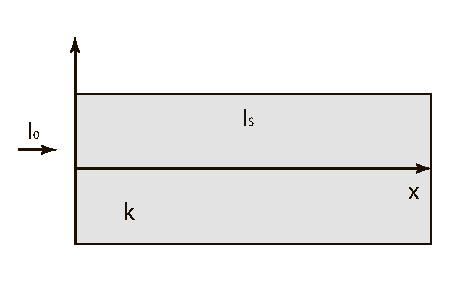
\includegraphics[width=.4\textwidth]{08_01}
\end{figure}

\[
	\begin{array}{c}
		dI = kI dx \\
		k = k(x); \quad I = I(x) \\
		\cfrac{dI}{dx} = kI; \quad k = \cfrac{k_0}{1-\cfrac{I}{I_s}} \\
		\cfrac{dI}{dx} = \cfrac{k_0 I}{1+\cfrac{I}{I_s}}; \quad
			\int\limits_{I_0}^{I} \cfrac{dI}{I}
			\left( 1 + \cfrac{I}{I_s} \right) = \int\limits_{0}^{x} k_0 dx \\
		\ln\cfrac{I}{I_0} + \cfrac{I}{I_s} - \cfrac{I_0}{I_s} = k_0 x \\
		\ln\cfrac{I}{I_0} = f(k_0 x) \text{ -- находится аналитически}
	\end{array}
\]

\begin{figure}[h!]
    \center
    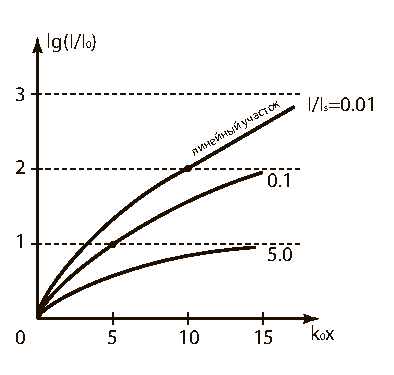
\includegraphics[width=.4\textwidth]{08_02}
\end{figure}

При малых уровнях интенсивности, когда \( I \ll I_s \) или \( I_0 \ll I_s \), 
вынужденное излучение не влияет на концентрацию частив в возбужденном 
состоянии. Тогда \( I(x) = I_0\exp(k_0 x) \) при 
\( I \gg I_s: \cfrac{\D I}{\D x} \simeq I_s k_0 \).

В этом случае практически вся энергия возбужденной среды переходит в энергию 
когерентного излучения. Скорость роста интенсивности стремится к постоянной 
величине.
\[
	I_s k_0 = \frac{h\nu\sigma N}{2\sigma\tau} = \frac{h\nu N}{2\tau} = const 
\]

\subquestion{Нерезонансные потери в активной среде}

1) Дифракционные
\begin{figure}[h!]
    \center
    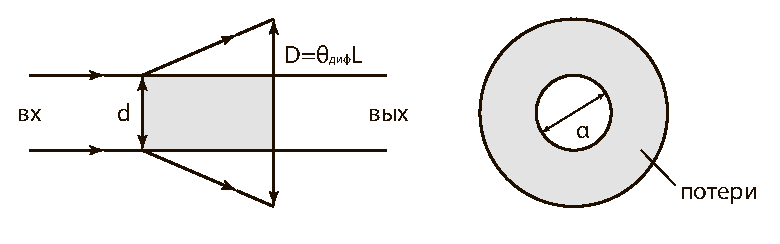
\includegraphics[width=.4\textwidth]{08_03}
\end{figure}
\[
	\theta_\text{диф} = 1.22\frac{\lambda}{d};\quad
	\eta_\text{диф} = (90\ldots99)\%
\]
2) На оптических элементах (многопроходный усилитель)
\begin{figure}[h!]
    \center
    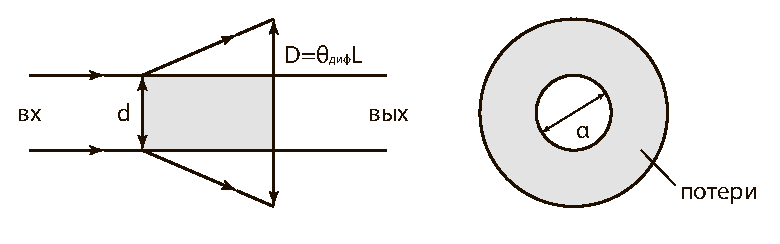
\includegraphics[width=.4\textwidth]{08_03}
\end{figure}
\[
	\eta_\text{нр} \approx 99\%
\]
3) На неоднородностях активной среды \\
Оптические неоднородности связаны с неоднородностью плотности (температуры, 
механического напряжения).